\documentclass[12pt,a4paper]{article}

\usepackage[T1]{fontenc}
\usepackage[utf8]{inputenc}
\usepackage[margin=2.5cm]{geometry}
\usepackage{graphicx}
\usepackage[hidelinks]{hyperref}
\usepackage{fancyhdr}
\usepackage{lastpage}
\usepackage{appendix}
\usepackage{amsmath}
\usepackage{color}
\usepackage{palatino}
\usepackage{changepage}
\usepackage{subcaption}
\usepackage{enumitem}
\usepackage{csquotes}
\usepackage{verbatim}
\usepackage[cache=false]{minted}

\usemintedstyle{fruity}

\title{Community detection in networks}
\author{Carlos Requena López}

%% Fancy layout
\pagestyle{fancy}
\lhead{INFO-F521}
\chead{}
\rhead{}
\lfoot{}
\cfoot{}
\rfoot{Page \thepage\ of \pageref{LastPage}}
\renewcommand{\headrulewidth}{0.4pt}
\renewcommand{\footrulewidth}{0.4pt}


%%% --- %%% --- DOCUMENT START --- %%% --- %%%
\begin{document}
\thispagestyle{fancy}
\maketitle
\thispagestyle{fancy}

\section{Introduction}

The topic of this assignment is community detection in networks by
means of hierarchical clustering. Informally, network communities can
be seen as dense (highly connected) subgraphs that are connected
between each other sparsely, only by few arcs or edges.

Hierarchical clustering (HC) refers to the technique of grouping
together elements that share some sort of similarity and separating
those that do not. HC can be \emph{divisive}, where elements start in
one cluster and are removed gradually or \emph{agglomerative}, where
every unit is its own cluster and are merged step by step.

\section{Analysis and expectations}

Let $ G = (V, E) $ be a simple, unweighted, undirected graph. Let $A$
be the adjacency matrix of $G$, defined as follows:

\[
  A_{ij} =
  \begin{cases}
    1 & \quad \text{if } (i,j) \in E\\
    0 & \quad \text{otherwise }
  \end{cases}
\]

We will use this adjacency matrix as the only source of information to
determine the similarity between vertices in the graph, but there
could be plenty of other sources depending on the application
domain. For example, when analysing text files, the similarity measure
could be the amount of equal significant words each one contains, or
in the case of aminoacids, the number of times it appears on protein
$p$ at location $l$.

Here, however, we compute the mean and variance between the rows of
the adjacency matrix as follows (if $A$ was not symmetric and $G$
undirected, it would have to be computed for rows \emph{and} columns):

$$ \mu_i = \frac{1}{n} \sum_{j=1}^{n} A_{ij} $$

$$ \sigma^2 = \frac{1}{n} \sum_{j=1}^{n} (A_{ij} - \mu_i)^2 $$

The similarity measure in this case is the Pearson product-moment
correlation coefficient:

$$ x_{ij} = \frac{\frac{1}{n}\sum_{k=1}^{n}(A_{ik} -
  \mu_i)(A_{jk}-\mu_j)}{\sigma_i\sigma_j} $$

All diagonal elements are excluded from these calculations
\cite[p.~369]{socionetwork}.

For example, for the simple graph given in
fig. \ref{fig:simple_graph}, the means, variances and similarity
measures are given in table

\begin{figure}[ht!]
  \centering
  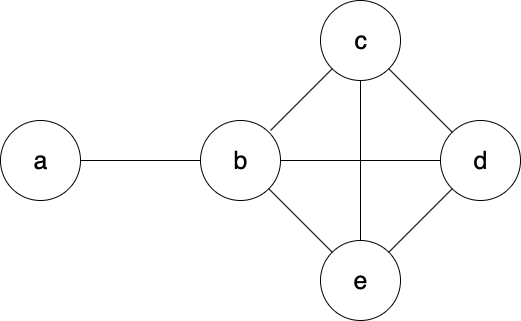
\includegraphics[width=0.6\textwidth]{img/simple_graph.png}
  \caption{Simple graph with 5 vertices}
  \label{fig:simple_graph}
\end{figure}



\section{Implementation}

The graph $ G $ is given as an adjacency matrix, which is parsed

\section{Results}

\section{Conclusion}

% \begin{figure}[ht!]
%   \centering
%   \includegraphics[width=1\textwidth]{some_graphic.png}
%   \caption{}
%   \label{fig:fig1}
% \end{figure}

\bibliographystyle{ieeetr}
\bibliography{main}
\nocite{*}

\appendix
\section{Appendix - code listing}

\inputminted{python}{../src/main.py}

% \begin{minted}{minted}
% \end{minted}


\end{document}
